\chapter{拉格朗日对偶性}

\textbf{Keyword.} \textsl{等式约束优化条件(拉格朗日乘子法)、不等式约束优化条件}

\section{拉格朗日乘子法}

考虑$n$元函数$f(x_1,x_2,\cdots,x_n)$的极值。一般情况下,函数极值的必要条件是
\begin{center}
    \textsl{$f$在极值点$r$的导数为$0$}
\end{center}

我们考虑约束下的函数极值问题
\begin{equation}
    \begin{aligned}
        & \min\limits_{x\in \mathbb{R}^n} f(x)\\
        & s.t.\ \ g(x)=c
    \end{aligned}
\end{equation}

拉格朗日乘数法的算法是
\begin{enumerate}[itemindent=2em]
    \item 首先构造拉格朗日函数
    \begin{equation}
        L(x,\lambda) = f(x)-\lambda g(x),\ \ \ x\in \mathbb{R}^n,\lambda\in \mathbb{R}
    \end{equation}
    \item 目的是求出使得拉格朗日函数的梯度为$0$的点
    \begin{equation}
        \triangledown L=\triangledown f(x)-\lambda\triangledown g=0
    \end{equation}
\end{enumerate}

解出上述方程即是极值问题的解。
\begin{figure}[H]
    \centering
    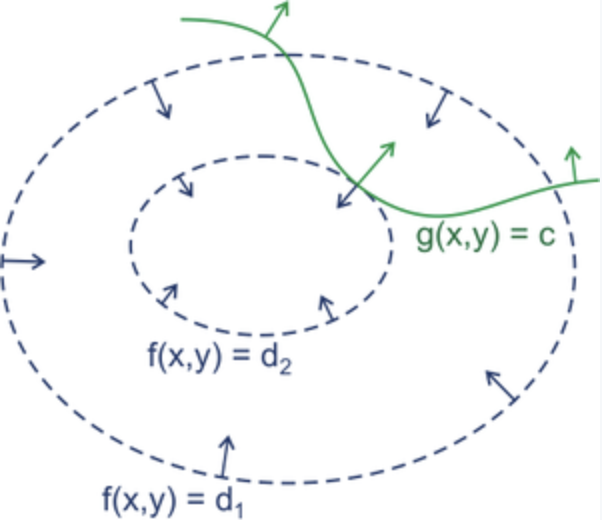
\includegraphics[scale=0.3]{figures/二元优化问题.png}
    \caption{拉格朗日乘子法的等高线图}
\end{figure}

根据等高线图,无约束下的极值点在$f(x,y)=d_2$内部,由于$g(x,y)=c$的约束使得只能取满足$g(x,y)=c$和$f(x,y)$的交点,
而交点中能使得$f(x,y)$取得最小值,正好是$f(x,y)=d_2$和$g(x,y)=c$的切点。而该点正好满足梯度方向相反,即存在$\lambda$
使得
\begin{equation}
    \triangledown f=\lambda\triangledown g
\end{equation}

因此原问题就变成了求拉格朗日函数的无约束极值问题。


\section{极小极大值问题(原始问题)}

假设$f(x),c_i(x),h_j(x)$是定义在$\mathbb{R}^n$上的连续可微函数。考虑优化问题
\begin{equation}
    \begin{aligned}
        & \min\limits_{x\in \mathbb{R}^n}\ f(x)\\
        & s.t. \ \ \ \ c_i(x)\leqslant 0,\ \ \ i=1,2,\cdots,k;\\
        &\ \ \ \ \ \ \ \  \ h_j(x)=0,\ \ \ j=1,2,\cdots,l;
    \end{aligned}
\end{equation}

引入拉格朗日函数

\begin{equation}
    L(x,\alpha,\beta)=f(x)+\sum\limits_{i=1}^{k}\alpha_ic_i(x)+\sum\limits_{j=1}^{l}\beta_jh_j(x)
\end{equation}

其中$x=(x^{(1)},x^{(2)},\cdots,x^{(n)})^T\in \mathbb{R}^n$,$\alpha_i,\beta_j$是拉格朗日乘子,
$\alpha_i\geqslant 0$。考虑
\begin{equation}
    \theta_P(x)=\max\limits_{\alpha,\beta,\alpha_i\geqslant 0} L(x,\alpha,\beta)
\end{equation}

其中下标$P$表示原始问题。

假设给定某个$x$,如果$x$违反原始问题的约束条件,即存在$i$使得$c_i(x)>0$或存在$j$使得$h_j(x)\neq 0$,则
\begin{equation}
    \theta_P(x)=\max\limits_{\alpha,\beta,\alpha_i\geqslant 0}
    [f(x)+\sum\limits_{i=1}^{k}\alpha_ic_i+\sum\limits_{i=1}^{l}\beta_jh_j(x)]=+\infty
\end{equation}

因为若$c_i(x)>0$,那么令$\alpha_i\rightarrow +\infty$,若$h_j(x)\neq 0$,则令$\beta_j$使得
$\beta_jh_j(x)\rightarrow +\infty$,其余将$\alpha_i,\beta_i$取为0即可。

因此
\begin{equation}
    \theta_P(x)=
    \begin{cases}
        & f(x),\ \ \ \ \mbox{x满足原始问题约束}\\
        & +\infty,\ \ \ else
    \end{cases}
\end{equation}

所以如果考虑极小化问题
\begin{equation}
    \theta_P(x)=\min\limits_{x}\max\limits_{\alpha,\beta,\alpha_i\geqslant 0} L(x,\alpha,\beta)
\end{equation}

它与原始优化问题是等价的,即解相同。问题$\min\limits_{x}\max\limits_{\alpha,\beta,\alpha_i\geqslant 0} L(x,\alpha,\beta)$
也被称为\textsl{广义拉格朗日函数的极小极大问题}。为了方便,定义原始问题为最优值
\begin{equation}
    p^*=\min\limits_{x}\theta_P(x)
\end{equation}

为原始问题的值。

\section{极大极小值问题(对偶问题)}
定义
\begin{equation}
    \theta_{D}(\alpha,\beta)=\min\limits_{x}L(x,\alpha,\beta)
\end{equation}

在考虑极大化$\theta_D(\alpha,\beta)$
\begin{equation}
    \max\limits_{\alpha,\beta,\alpha_i\geqslant 0}\theta_{D}(\alpha,\beta)= \max\limits_{\alpha,\beta,\alpha_i\geqslant 0}\min\limits_{x}L(x,\alpha,\beta)
\end{equation}

这样的问题称为\textsl{广义拉格朗日函数的极大极小问题}

可以将广义拉格朗日函数的极大极小问题表示为约束最优化问题:
\begin{equation}
    \begin{aligned}
        & \max\limits_{\alpha,\beta,\alpha_i\geqslant 0}\theta_{D}(\alpha,\beta)= \max\limits_{\alpha,\beta,\alpha_i\geqslant 0}\min\limits_{x}L(x,\alpha,\beta)\\
        & \ \ \ s.t. \ \ \ \ \ \alpha_i\geqslant 0,\ \ \ i=1,2,\cdots,k
    \end{aligned}
\end{equation}

称为原始问题的对偶问题,定义对偶问题的最优值
\begin{equation}
    d^*=\max\limits_{\alpha,\beta,\alpha_i\geqslant 0} \theta_D(\alpha,\beta)
\end{equation}

称为对偶问题的值。

\section{原始问题和对偶问题的关系}

\begin{theorem}
    若原始问题和对偶问题都有最优值,则
    \begin{equation}
        d^*=\max\limits_{\alpha,\beta,\alpha_i\geqslant 0} \theta_D(\alpha,\beta)
        \leqslant \min\limits_{\alpha,\beta,\alpha_i\geqslant 0} \theta_P(\alpha,\beta)=p^*
    \end{equation}
\end{theorem}

\textbf{proof. } 对任意的$\alpha,\beta$和$x$,有
\begin{equation}
    \theta_D(\alpha,\beta)=\min\limits_{x}L(x,\alpha,\beta)\leqslant L(x,\alpha,\beta)
    \leqslant \min\limits_{x}\max\limits_{\alpha,\beta,\alpha_i\geqslant 0}L(x,\alpha,\beta)=p^*
\end{equation}

即
\begin{equation}
    \theta_D(\alpha,\beta)\leqslant \theta_P(x)
\end{equation}

由于原始问题和对偶问题都有最优值
\begin{equation}
    \max\limits_{\alpha,\beta,\alpha_i\geqslant 0}\theta_D(\alpha,\beta)\leqslant \min\limits_{x}\theta_P(x)
\end{equation}

$\Box$

\begin{corollary}
    设$x^*$和$\alpha^*,\beta^*$分别是原始问题和对偶问题的可行解,并且$d^*=p^*$,则$x^*$和$\alpha^*,\beta^*$分别是
    原始问题和对偶问题的最优解。
\end{corollary}

\begin{theorem}
    考虑原始问题和对偶问题。假设函数$f(x)$和$c_i(x)$是凸函数,$h_j(x)$是仿射函数;并且假设不等式约束$c_i(x)$是严格可行的,
    即存在$x_i$对所有的$i$有$c_i(x)<0$,则存在$x^*,\alpha^*,\beta^*$,使得$x^*$是原始问题的解,$\alpha^*,\beta^*$是
    对偶问题的解,并且
    \begin{equation}
        p^*=d^*=L(x^*,\alpha^*,\beta^*)
    \end{equation}
\end{theorem}

\section{KKT条件}
\begin{theorem}
    对原始问题和对偶问题。假设函数$f(x)$和$c_i(x)$是凸函数,$h_j(x)$是仿射函数;并且不等式约束$c_i(x)$是严格可行的,
    则$x^*$和$\alpha^*,\beta^*$分别是原始问题和对偶问题的解的充分必要条件是:$\alpha^*,\beta^*,x^*$满足下面的
    \textsl{\textbf{Karush-Kuhn-Tucker条件}(KKT)}
    \begin{equation}
        \bigtriangledown_x L(x^*,\alpha^*,\beta^*)=0
    \end{equation}
    \begin{equation}
        \alpha^*_ic_i(x^*)=0,\ \ \ i=1,2,\cdots,k
        \label{C.22}
    \end{equation}
    \begin{equation}
        c_i(x^*)\leqslant 0,\ \ \ i=1,2,\cdots,k
    \end{equation}
    \begin{equation}
        \alpha^*_i\geqslant 0,\ \ \ i=1,2,\cdots,k
    \end{equation}
    \begin{equation}
        h_j(x^*)=0,\ \ \ i=1,2,\cdots,l
    \end{equation}
\end{theorem}

其中(\ref{C.22})是KKT的\textsl{\textbf{对偶互补条件}}。由此条件,若$\alpha^*_i>0$,则$c_i(x^*)=0$

